\documentclass[12pt]{article}

\usepackage{amsmath,amssymb,amsthm}
\usepackage[T1]{fontenc}
\usepackage{graphics}
\usepackage{qtree}
\usepackage{tikz}
\usepackage[utf8]{inputenc} % æøå
\usepackage[T1]{fontenc} % mere æøå
\usepackage[danish]{babel} % orddeling
\usepackage{verbatim} % så man kan skrive ren tekst
\usepackage[all]{xy} % den sidste (avancerede) formel i dokumentet
\usepackage{fullpage} % mindre margin

\title{ProjDat 2014\\Props 2.0}
\author{Louise Knudsen (140791 - zsh845)\\
Helena Bach (180492 - wzg314)\\
David Pedersen (060890 - tlb209)\\\\
Instructor: Simon Shine }
\date{\today}

\newcommand{\R}{\mathbb{R}}
\newcommand{\C}{\mathbb{C}}
\newcommand{\N}{\mathbb{N}}
\newcommand{\Z}{\mathbb{Z}}
\newcommand{\Q}{\mathbb{Q}}

\newcommand{\og}{\wedge}

\begin{document}
\maketitle
\newpage
\section{Problem definition}
\textit{The Royal Danish Theatre's props department uses a locally installed database-system to search through all of the props and productions and their corresponding set-up- and run-lists. The system was developed more than 20 years ago by their own Claus Nepper Fakkenberg. Claus alone holds the responsibility for maintaining the system, as he is the only one who understands the source-code, which will soon be a problem as he is now retiring. \\
Due to the age of the system, some functionalities are no longer needed, and there are new requirements that are not implemented, most importantly a need to use the system outside of the office.} \\\\
The problem can be described with the following points:
\begin{itemize}
  \item The current database system was developed in 1989, and lacks a lot of wanted functionalities.
  \item The developer, Claus, is the only one who can modify and support the system.
  \item Claus is retiring.
\end{itemize}
To analyze the problems defined above and develop a system definition we use the FACTOR Criterion.
\subsection{The FACTOR Criterion}
\begin{description}
  \item[Functionality:] Keeping track of the props and performances, and help in running these. As well as support the administration.
  \item[Application domain:] The Royal Danish Theatre.
  \item[Conditions:] The system should be usable by multiple user at a time, wherever there are access to the internet.
  \item[Technology:] The system will be developed on standard laptops, and should be usable on standard PC's and tablets and supported by every OS.
  \item[Object:] Props, pictures and employees in the props department.
  \item[Responsibility:] Searching and administrative tool.
\end{description}
\subsection{System definition}
A web-based database-system of The Royal Danish Theatre props department. The system should primarily be a searching tool used to prepare and run performances and search for props in current and previous productions by the assistant stage managers, and secondly be used for budget monitoring, search for supplier information as well as keeping track of all performance information, by the chairman of the props department. The system should be usable for people with greatly variable computer experience.
\subsection{Requirements}
We have had multiple meetings with the different people who have daily contact with the system to form a idea of the needs and requirements, but only April 9th these will be formalised more specifically, when we kick off the project in collaboration with the client.
\subsection{Constraints}
The constraints of our project include the security aspect, which the head of the IT-department, Martin Thaarup Larsen, makes sure to handle in a way that makes it possible for our system to be part of the existing login-system. Martin has the responsibility for the media database as well - most likely made accessible to us through a "mirror database".   
\subsection{Solution domain}
The solution domain can be defined as being the props department as well as Cumulus, their media database, which our application will be interfacing with.
\subsection{Deliverables}
\begin{itemize}
  \item PHP code
  \item MySQL database
  \item Instructions in the form of meetings in addition to papers explaining the system.
  \item Probably also some support during the initial start up phase.
\end{itemize}
\section{Initial Software Project Management Plan}
\subsection{Overview of the project}
To give a initial overview of the project in terms of planning and managing we have composed the following points.
\subsubsection{Project summary}
\underline{Work product:} \\
- MySQL database \\
- PHP code for the web-interface. \\
- Assignments describing the work process\\\\
\underline{Schedule:} \\
On April 9th we are scheduled to meet with Martin and Mikkel from the theatre, to finalize the requirements elicitation and sign the project agreement. We will thereafter be able to put together a more detailed time-schedule.\\
On June 23rd we have our final deadline, and will hopefully deliver the final product to the theatre. \\\\
\underline{Participants:}\\
Developers: David Pedersen, Helena Bach, Louise Knudsen \\
Project managers: David Pedersen, Helena Bach, Louise Knudsen \\
Client: The Royal Danish Theatre.\\\\
\underline{Tasks:} \\
The developers will have a common responsibility to participate in every aspect of the system-development. Of course their will be a natural division of the task in correspondence to each developers skill- and interest-level as described in the skill matrix, which is found in section 5. 
\subsubsection{Evolution of the plan}
All changes to the project management plan must be agreed to by all participants before they are implemented. All changes should be documented in the, to the developers, shared log, and in time become a part of the final SPMP.
\subsection{References}
All artifacts will conform to the theatres standards.
\subsection{Definitions}
The Royal Danish Theatre uses a lot of different terms in their work, and some of these should also be used in the future database system. The terms we have been presented to so far are listed with a short description below: \\
Every production has a unique 8-digit number, containing of 4 random digits followed by a dash and premiere-year for this particular production. (There can be multiple productions of, for instance the same play, which then have different premiere-years) \\
If a production is \textit{SKILT}, it means that it has been discarded and the props are back in the storage room. \\
If a production is \textit{I REPERTOIRE}, it is being played in the current season and the props are in use. \\
If the production is \textit{I CONTAINER} or similar, the production is not yet \textit{SKILT} nor is it currently being played, and the props are therefore occupied but not in use.
\subsection{Project Organization}
\subsubsection{External interfaces}
The props database and appertaining web-interface will be managed and developed by David Pedersen, Helena Bach and Louise Knudsen. \\
The photographs of the props and productions, along with the login system and server connection will be handled by Martin. \\
All managers will be in continuous contact with the chairman of the props department, Mikkel Rasmus Theut, as well as Martin.\\\\
During the project we will be communication primarily with these people for feedback and questions.
\begin{itemize}
  \item Mikkel Theut: Chairman of the props department.
  \item Martin Thaarup Larsen: Head of the IT-department.
  \item Palle Henriksen: Head of the furniture subdivision.
  \item Thomas Kolding: Employed at the furniture subdivision.
  \item Charlotte: Employed at the theatre. She is responsible for adding new props to the database.
\end{itemize}
\subsection{Managerial process plans}
\subsubsection{Start-up plan}
The total developments time is estimated to be 15 week, counting from 13/03/2014, where first meeting with the client was held. \\
All necessary hardware are available, as well are the software since MySQL and PHP both are open-source.
\subsubsection{Work plan}
\underline{Week 1-5:}
\begin{itemize}
  \item Initial meeting with Mikkel.
  \item More technically oriented meeting with Martin where Mikkel were also present.
  \item Meeting with head of the furniture subdivision.
  Prepare the requirements elicitation and the Project Agreement.
  \item Meeting with Martin and Mikkel - signing of the requirements elicitation and the Project Agreement, and project kick-off!
\end{itemize}
\underline{Week 6-7:}
\begin{itemize}
  \item Focus on making the SQL-script.
\end{itemize}
\underline{Week 8-11:}
\begin{itemize}
  \item Finish SQL.
  \item Start design of the web-application.
  \item Begin PHP-coding and testing.
\end{itemize}
\underline{Week 12-15:}
\begin{itemize}
  \item Finish PHP-coding and testing.
  \item Final documentation.
\end{itemize}
% \subsubsection{Control plan}
\subsubsection{Risk management plan}
The risk factors and the tracking mechanisms are as follows. \\\\
As one of the goals of the project is to achieve more functionality than the existing system, there should in the testing-process be compared results between the two. \\\\
There should in the designing-process be a great amount of communication with the client to ensure an as user-friendly interface as possible, as the system mainly will be used by people with limited computer-experience. \\\\
There is a slim chance of hardware failure, in which case each developer is responsible for there own computer, and the client holds the responsibility for the server. \\\\
Each developer is responsible for continuous testing of their assigned subsystem(s) and jointly cross-testing between these. 
% \subsubsection{Closeout plan}
\subsection{Techinical process plans}
We are not far enough along in the process to be able to make any decisions here.
%\subsubsection{Process model}
%\subsubsection{Methods, tools, and techniques}
%\subsubsection{Infrastructure}
%\subsubsection{Product acceptance plan}
\subsection{Supporting process plans}
\subsubsection{Configuration management plan}
Git and GitHub will be used in all aspects of the project to ensure version control.\\\\
We are not far enough along in the process to be able to make any further decisions here.
% \subsubsection{Verification and validation plan}
% \subsubsection{Documentation plan}
% \subsubsection{Quality assurance plan}
% \subsubsection{Reviews and audits}
% \subsubsection{Problem resolution plan}
% \subsubsection{Subcontractor management plan}
% \subsubsection{Process improvement plan}
\subsection{Additional plans}
\subsubsection{Presentation}
In connection with the delivery of the final product, the system and its functionalities will be a presented to the chairman of the props department, Mikkel. \\
As one of the purposes of developing the new system, is to make it possible for the head of the IT-department, Martin, to keep the system up to date himself, we will in addition to the presentation, be going through code with him.
\subsubsection{Support}
During the initialisation phase support will be offered free of charge.
\section{Initial software architecture}
\subsection{Design goals}
First of we would like to note that this architecture is in a very early phase
and will most likely change as we move forward in the process.\\
Given the circumstances that this application will be built and deployed under (namely that we might not be the ones who end up maintaining it) it is important for the design of the system to be well documented and well structured.\\\\
We have the following overall design goals for the system:
\begin{itemize}
  \item The system should be factored into meaning full subsystems each with a well defined responsibility.
  \item The system should make use of both unit and integration level tests as this will allow for easier refactoring and maintenance of the system. This is especially important since we might not be the ones who will be responsible for maintaining the system.
\end{itemize}
\subsection{Initial system design}
\subsubsection{Subsystem decomposition}
At this early stage in the process it is hard to say which subsystems there will be. However there will likely be some subsystems that are responsible for talking with the external systems that manage the media database and user authorization.

Given that our application will most likely be a website backed by a relation database there will be three primary layers to it:

\begin{enumerate}
  \item The database.
  \item The domain model.
  \item The web front end.
\end{enumerate}
Each layer will have their own responsibility.
\subsubsection{The database}
Here all data will be stored. It will most likely be some sort of relation database.
\subsubsection{The domain model}
In web terms this will be the back end of the website. This is where domain
concepts such as props and performances are given attributes and methods that
given them behavior and allow them to interact with each other and the user.
This is also where important features of the application will be modeled such as
how a search can be performed on the database.
\subsubsection{The web front end}
This layer will be a graphical representation of the data and relationships
between the different data points built by the back end. This is also the part
of application that the end user will interact with. \\
Since we are building a web application this layer will be built using the
standard set of web technologies, HTML, CSS, and JavaScript.\\
Each of these three subsystems will each be composed of their own smaller
subsystems that each have a well defined purpose and responsibility.
\subsubsection{MVC}
For decomposing the back and front end and the relationships between them we
have chosen to use the MVC design pattern. This lets us split the system up into
small manageable parts with a clear purpose and responsibility. This will make
the code more maintainable and more suitable to change.
Depending on the domain your application lives in the separation and
responsibilities of the models, controllers, and views might be slightly
different. Here are some initial thoughts about what each subsystem will be
responsible for.
\subsubsection{Model}
The model layer will contain code that models the entities in the domain. For
our application there will most likely be a props models, a performance/play
model and others.\\
This is also the layer that is responsible for communicating with the database
and managing the persistence of the objects.
\subsubsection{View}
The view layer will contain the graphical representation of the model layer that
the user can view and interact with.
\subsubsection{Controller}
The controller layer is responsible to managing the interactions that the user
makes with the model layer. A user will be performing actions like navigating
between pages, submitting forms, searching for props, and so on. It will be the
controllers responsibility to map these actions into the model layer and
construct new views for the user. It essentially acts as glue code between the
user and the domain/model layer.

\subsubsection{Dependencies}
The MVC design pattern is very useful for managing and limiting dependencies
between the different subsystems. An important part of MVC is that the model
layer and view layer should be as little dependent on each other as possible.
This will make it easier to change each part independently.\\
It is however not possible to make the controllers free of dependencies since
they sit in between the views and the model. Therefor they are naturally
dependent on both the views and the model. However MVC helps with this by
providing each subsystem with single responsibility thus making each of them
smaller and more well defined.\\
The system will also have to interact with other external systems. This will
primarily be Cumulus for linking a prop in our system with pictures in the media
database.
\subsection{Initial subsystem components}
\subsubsection{Views}
At this early point it is hard to say which views the application will contain
but there will likely be views related to the following areas:

\begin{itemize}
  \item View that lists props. This could be a listing of all props in the database but more likely a list filtered based on some search criteria.
  \item View for doing a search. This view would contain a form with fields for filtering through the props.
  \item View the shows a specific prop. There will most likely be a view that shows the information available about a single prop and its relationships.
  \item Administrative views. These would be views that let administrators perform usual operations on the data (create new, update existing, and delete existing).
\end{itemize}

\subsubsection{Models}
Given the views listed above our model layer will most likely include:

\begin{itemize}
  \item User model. If the application ends up containing authentication and users with different roles then there will also be a model responsible for that behavior.
  \item Prop model. Given that this application is about props there will most certainly be a prop model that describes the properties and behavior of props.
  \item Performance model. If props need to be related to performances then there will also be a performance model.
\end{itemize}
Given that it should be possible to persist the model objects in the database
there will need to a subsystem that handles that. It also makes sense for this
system to be responsible for building model objects from the data in the
database. Exactly how this will be modeled is too early to say but given that
this is behavior is shared between all the models it might be modeled with
inheritance or object composition.
\subsubsection{Controllers}
Specifically which controllers the system will include depend on which views we
want and how they are grouped together. However since this application is
primarily about searching there will most likely be a controller that is
responsible for receiving a search query, then translating that to a query the
model layer can perform and then rendering a view containing the results to the
user.

\subsection{Diagrams}
Here is a class diagram of the model layer as we imagine it might look.
\newline
\newline
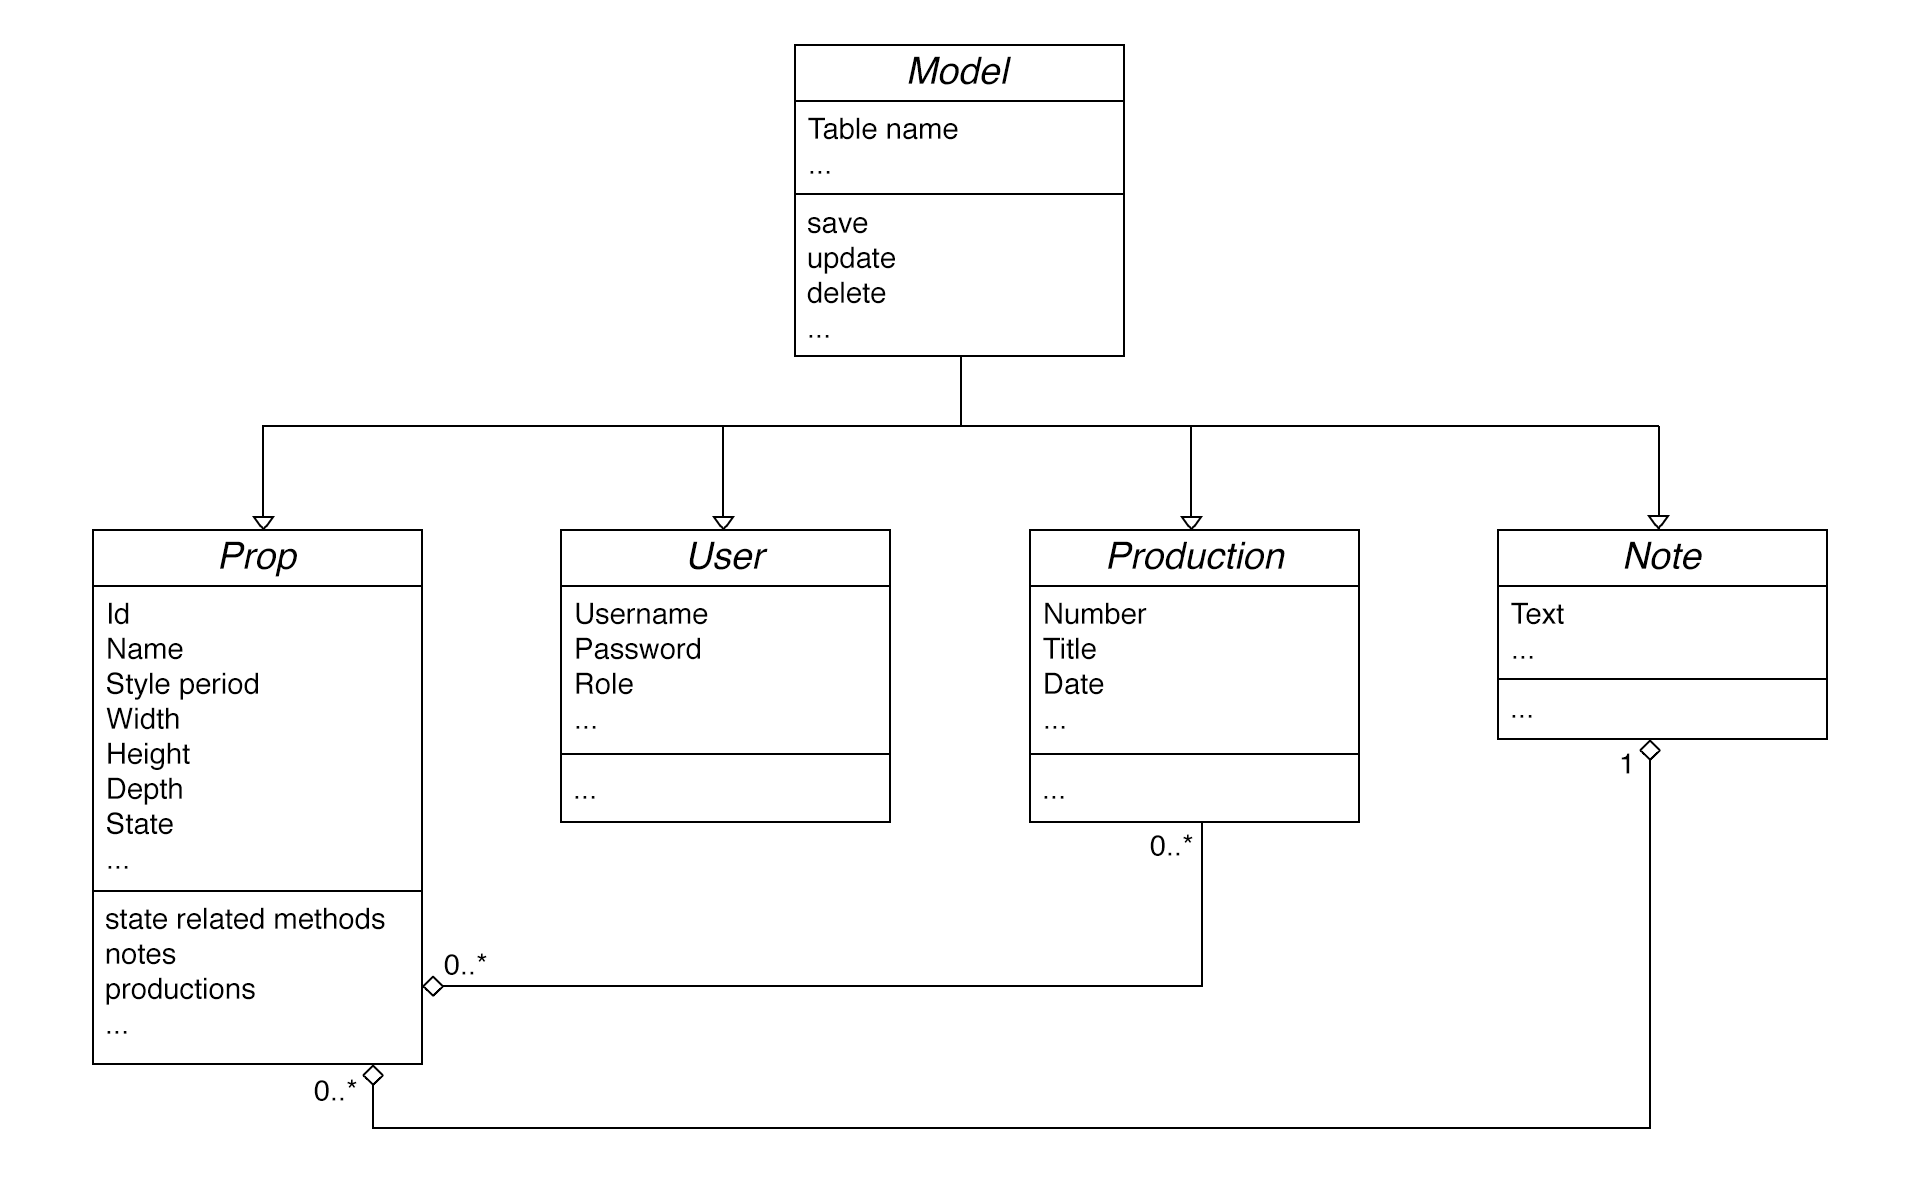
\includegraphics[scale=0.2]{class-diagram.png}

\section{Project Agreement definition}
As mentioned in previous sections our final requirement elicitation and project agreement will be formalized on April 9th, at our meeting with Mikkel and Martin. To prepare for the meeting and make an outline for this final definition we have made the following UML use case diagram (See Appendix A for use cases) and functional/nonfuntional requirements overview.
\subsection{UML use case diagram}
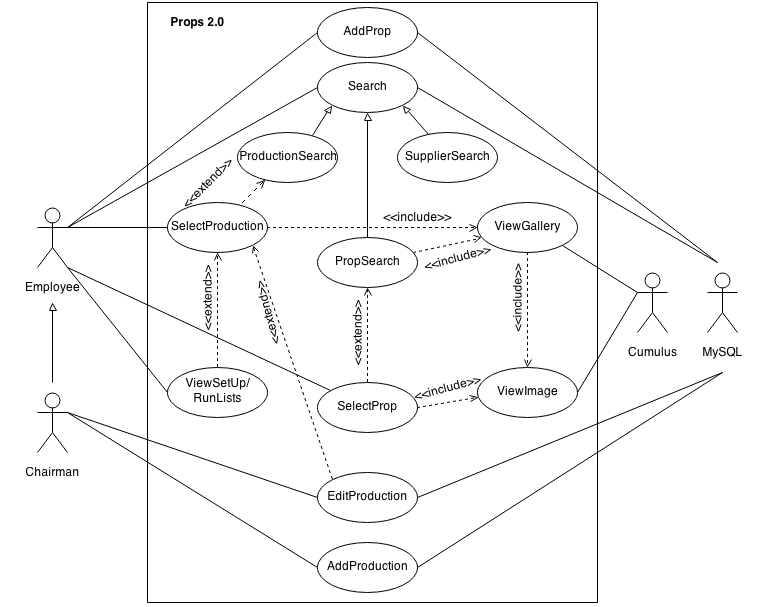
\includegraphics[scale=0.6]{use.png}
\subsection{Nonfunctional Requirements}
\begin{itemize}
  \item The system should be web-based and usable on standard PC's and tablets, and supported by every OS.
  \item The webapplication should be user friendly and easy to navigate. The most commonly used functionalities, namely the run- and set-up-lists should not be more than 3 clicks away.
  \item It should be possible for Martin to maintain and support, and possibly expand the system after product-delivery. Therefore the system will be developed using MySQL and PHP, which is familiar to Martin.
  \item The system should be able to communicate with the existing media-database Cumulus.
  \item The system should be secure in a way that prevents people from the outside to corrupt the data.
  \item The interface should be in Danish.
  \item It should be made in such a way that makes it easy to extend with additonal functionality.
\end{itemize}
\subsection{Functional Requirements}
\begin{itemize}
  \item It should be possible to do cross search for props, productions, and suppliers.
  \item It should be possible to add, edit and delete props, productions, and suppliers.
  \item It should be possible to print run- and set-up-lists.
\end{itemize}
\section{Internal project establishment}
To get an overview of the participants skill set and learn who could be responsible for which subsystems we made a skill matrix.\\

$\bullet$ = Primary skill \quad $\bigcirc$ = secondary skill \quad $\bigtriangleup$ = interest.
\[
\begin{array}{|l|l|l|l|}
\hline
\textbf{Tasks/Participant} & David & Helena & Louise\\
\hline
\text{Database Design} & \bigcirc & \bullet & \bullet\\
\hline
\text{Web Programming} & \bullet & \bigtriangleup & \bigtriangleup\\
\hline
\text{Testing} & \bullet \bigtriangleup & & \\
\hline
\text{UI Design} & \bigtriangleup & \bigtriangleup & \bullet \bigtriangleup\\
\hline
\text{Project Management} & & \bullet & \bigcirc\\
\hline
\text{Object oriented programming} & \bullet \bigtriangleup& \bigcirc \bigtriangleup & \bigcirc \\
\hline
\end{array}
\]
When the subsystems get defined, we can now use this matrix to delegate the tasks and responsibilities in the most suitable and efficient way.
\section{Appendices}
\subsection{Appendix A: Use cases}
%1. Tilføj Rek
\[
\begin{array}{ll}
\hline
\textit{Use case name} & \texttt{AddProp} \\
\hline
\textit{Participating actors} & \text{Initiated by \texttt{Employee}} \\
& \text{Communicates with \texttt{MySQL}} \\
\hline
\textit{Flow of events} & 
\begin{array}{l}
\text{1. The \texttt{Employee} activates the "Add prop"  function.}\\
\quad \quad \quad \text{2. \texttt{Props 2.0} responds by presenting a form to the \texttt{Employee}.} \\
\text{3. The \texttt{Employee} fills out the form with the relevant prop-info,} \\ \quad \text{and submits it.} \\
\quad \quad \quad \text{4. \texttt{Props 2.0} receives the form, and the MySQL database} \\ \quad \quad \quad \quad \text{gets updated. \texttt{Props 2.0} displays a confirmation of the}\\ \quad \quad \quad \quad \text{update.}
\end{array} \\
\hline
\textit{Entry condition} & \text{The \texttt{Employee} must be logged into the Theatre's Wi-Fi} \\
\hline
\textit{Exit condition} & \text{The \texttt{Employee} has received a confirmation OR} \\ & \text{An explanation indicating why the transaction could not be processed.} \\
\hline
\textit{Quality requirements} & \text{Not yet defined} \\
\hline
\end{array}
\]
%2. Tilføj forestilling
\\
\\
\[
\begin{array}{ll}
\hline
\textit{Use case name} & \texttt{AddProduction} \\
\hline
\textit{Participating actors} & \text{Initiated by \texttt{Chairman}} \\
& \text{Communicates with \texttt{MySQL}} \\
\hline
\textit{Flow of events} & 
\begin{array}{l}
\text{1. The \texttt{Chairman} activates the "Add production" function.}\\
\quad \quad \quad \text{2. \texttt{Props 2.0} responds by presenting a form to the \texttt{Chairman}.} \\
\text{3. The \texttt{Chairman} fills out the form with the relevant production-info,} \\ \quad \text{and submits it.} \\
\quad \quad \quad \text{4. \texttt{Props 2.0} receives the form, and the MySQL database} \\ \quad \quad \quad \quad \text{gets updated. \texttt{Props 2.0} displays a confirmation of the}\\ \quad \quad \quad \quad \text{update.}
\end{array} \\
\hline
\textit{Entry condition} & \text{The \texttt{Chairman} must be logged into the Theatre's Wi-Fi} \\
\hline
\textit{Exit condition} & \text{The \texttt{Chairman} has received a confirmation OR} \\ & \text{An explanation indicating why the transaction could not be processed.} \\
\hline
\textit{Quality requirements} & \text{Not yet defined}\\
\hline
\end{array}
\]
%3. Søg
\\
\\
\[
\begin{array}{ll}
\hline
\textit{Use case name} & \texttt{Search} \\
\hline
\textit{Participating actors} & \text{Initiated by \texttt{Employee}} \\
& \text{Communicates with \texttt{MySQL}} \\
\hline
\textit{Flow of events} & 
\begin{array}{l}
\text{1. The \texttt{Employee} activates the "Search" function.}\\
\quad \quad \quad \text{2. \texttt{Props 2.0} responds by presenting a form to the \texttt{Employee}.} \\
\text{3. The \texttt{Employee} fills out the form with the search criteria,} \\ \quad \text{and submits it.} \\
\quad \quad \quad \text{4. \texttt{Props 2.0} receives the form, the MySQL database} \\ \quad \quad \quad \quad \text{returns the matching data and \texttt{Props 2.0} displays it}
\end{array} \\
\hline
\textit{Entry condition} & \text{The \texttt{Employee} must be logged into the Theatre's Wi-Fi} \\
\hline
\textit{Exit condition} & \text{The \texttt{Employee} has received a list of matching data OR} \\ & \text{A "No match"  message} \\
\hline
\textit{Quality requirements} & \text{Not yet defined} \\
\hline
\end{array}
\]
We have not yet fully specified the search criteria with the client. We know that separate search-functions for productions, props and suppliers are wanted, but until we have the detailed criteria, we will not include these as specific use cases.  
%4. Vælg rek
\\
\\
\[
\begin{array}{ll}
\hline
\textit{Use case name} & \texttt{SelectProp} \\
\hline
\textit{Participating actors} & \text{Initiated by \texttt{Employee}} \\
\hline
\textit{Flow of events} & 
\begin{array}{l}
\text{1. The \texttt{Employee} selects a prop from the results of a premade search} \\
\quad \quad \quad \text{2. \texttt{Props 2.0} responds by presenting a more detailed}\\ \quad \quad \quad \quad \text{description of the prop to the \texttt{Employee}.}
\end{array} \\
\hline
\textit{Entry condition} & \text{This use case extends the  \texttt{PropSearch} use case} \\
\hline
\textit{Exit condition} & \text{The \texttt{Employee} is looking at the prop description} \\
\hline
\textit{Quality requirements} & \text{This use case includes the \texttt{ViewImage} use case} \\
\hline
\end{array}
\]
%5. Vælg forestilling:\\
\\
\\
\[
\begin{array}{ll}
\hline
\textit{Use case name} & \texttt{SelectProduction} \\
\hline
\textit{Participating actors} & \text{Initiated by \texttt{Employee}} \\
\hline
\textit{Flow of events} & 
\begin{array}{l}
\text{1. The \texttt{Employee} selects a production from the results of a premade}\\ \quad \text{search}\\
\quad \quad \quad \text{2. \texttt{Props 2.0} responds by presenting a more detailed}\\
\quad \quad \quad \quad \text{description of the production to the \texttt{Employee}.}
\end{array} \\
\hline
\textit{Entry condition} &
\text{This use case extends the \texttt{ProductionSearch} use case.}\\
\hline
\textit{Exit condition} & \text{The \texttt{Employee} is looking at the production information.} \\
\hline
\textit{Quality requirements} & \text{This use case includes the \texttt{ViewGallery} use case.} \\
\hline
\end{array}
\]
%6. Køre/opstil
\\
\\
\[
\begin{array}{ll}
\hline
\textit{Use case name} & \texttt{ViewSetUp/RunLists} \\
\hline
\textit{Participating actors} & \text{Initiated by \texttt{Employee}} \\
\hline
\textit{Flow of events} & 
\begin{array}{l}
\text{1. The \texttt{Employee} selects the list from the results of a production} \\ \quad \text{search} \\
\quad \quad \quad \text{2. \texttt{Props 2.0} responds by presenting the list to the}\\ \quad \quad \quad \quad \texttt{Employee.}
\end{array} \\
\hline
\textit{Entry condition} & \text{This use case extends the  \texttt{SelectProduction} use case} \\
\hline
\textit{Exit condition} & \text{The \texttt{Employee} is looking at the list} \\
\hline
\textit{Quality requirements} & \text{Not yet defined} \\
\hline
\end{array}
\]
%7. Redigér/slet
\\
\\
\[
\begin{array}{ll}
\hline
\textit{Use case name} & \texttt{EditProduction} \\
\hline
\textit{Participating actors} & \text{Initiated by \texttt{Chairman}} \\
& \text{Communitates with \texttt{MySQL}} \\
\hline
\textit{Flow of events} & 
\begin{array}{l}
\text{1. The \texttt{Chairman} activates the "Edit production" function} \\
\quad \quad \quad \text{2. \texttt{Props 2.0} responds by presenting a form to the \texttt{Chairman}}\\
\text{3. The \texttt{Chairman} fills out the form and submit the changes OR} \\ \quad \text{The \texttt{Chairman} selects the "Delete" option} \\
\quad \quad \quad \text{4. \texttt{Props 2.0} receives the form, and the MySQL database} \\ \quad \quad \quad \quad \text{gets updated. \texttt{Props 2.0} displays a update- OR}\\\quad \quad \quad \quad \text{delete-comfirmation} 
\end{array} \\
\hline
\textit{Entry condition} & \text{This use case extends the  \texttt{SelectProduction} use case} \\
\hline
\textit{Exit condition} & \text{The \texttt{Chairman} has received a confirmation OR} \\ & \text{An explanation indicating why the transaction could not be processed.} \\
\hline
\textit{Quality requirements} & \text{Not yet defined} \\
\hline
\end{array}
\]
%8. Se Galleri:
\\
\\
\[
\begin{array}{ll}
\hline
\textit{Use case name} & \texttt{ViewGallery} \\
\hline
\textit{Participating actors} & \text{Initiated by \texttt{Employee}}\\ &
\text{Communicates with \texttt{Cumulus}}\\
\hline
\textit{Flow of events} & 
\begin{array}{l}
\text{1. The \texttt{SelectProduction} or \texttt{PropSearch} use case gets evoked}\\
\quad \quad \quad \text{2. \texttt{Props 2.0} requests \texttt{Cumulus} for the image data}\\
3.\text{\texttt{Cumulus} returns the matching images}\\
\quad \quad \quad \text{4. \texttt{Props 2.0} responds by presenting the images as a gallery}
\end{array} \\
\hline
\textit{Entry condition} &
\text{The \texttt{Employee} must initiate the \texttt{SelectProduction} or \texttt{PropSearch}}\\ &
\text{use case to initiate this use case}\\
\hline
\textit{Exit condition} & \text{The \texttt{Employee} is looking at the gallery.} \\
\hline
\textit{Quality requirements} & \text{This use case includes the \texttt{ViewImage} use case.} \\
\hline
\end{array}
\]
%9. Se billede:
\\
\\
\[
\begin{array}{ll}
\hline
\textit{Use case name} & \texttt{ViewImage} \\
\hline
\textit{Participating actors} & \text{Initiated by \texttt{Employee}}\\ &
\text{Communicates with \texttt{Cumulus}}\\
\hline
\textit{Flow of events} & 
\begin{array}{l}
\text{1. The \texttt{ViewGallery} or \texttt{SelectProp} use case gets evoked}\\
\quad \quad \quad \text{2. \texttt{Props 2.0} requests \texttt{Cumulus} for the image}\\
\text{3. \texttt{Cumulus} returns the matching image}\\
\quad \quad \quad \text{4. \texttt{Props 2.0} responds by presenting the image to the}\\ \quad \quad \quad \quad\texttt{Employee}
\end{array} \\
\hline
\textit{Entry condition} &
\text{The \texttt{Employee} must initiate the \texttt{ViewGallery} or \texttt{SelectProp} use}\\ &
\text{case to initiate this use case}\\
\hline
\textit{Exit condition} & \text{The \texttt{Employee} is looking at the image.} \\
\hline
\textit{Quality requirements} & \text{Not yet defined} \\
\hline
\end{array}
\]
\end{document}
